\section*{Multiple-choice}\label{sec:mc}

Dine svar skal indtastes i ITX-systemets multiple-choice modul.

\multiplechoicestart


\spoergsmaal{Asymptotiske grænser}
Nedenfor er angivet et antal udtryk for køretid. Hvilken køretid er asymptotisk langsomst voksende?
\etsvar
\mulighederstart
\svar{$n^2 + n \log n$}
\svar{$n^{\log_2(3)} + 1000\, n$}
\svar{$n \log n + \sqrt{n}$}
\svar{$2^n + n^{100}$}
\svar{$\log(4^n)$}\korrekt
\mulighederslut
\forklaring{
Vi sammenligner ved at forenkle hvert udtryk til dets dominerende led:
\[
n^2+n \log n=\Theta(n^2), \qquad
n^{\log_2 3}+1000\, n=\Theta(n^{\log_2 3}),
\]
\[
n \log n+\sqrt{n}=\Theta(n \log n), \qquad
2^n+n^{100}=\Theta(2^n).
\]
\[
\log(4^n)=n \log 4=\Theta(n).
\]
Den langsomst voksende (og dermed hurtigste) er $\Theta(n)$, altså $\log(4^n)$.
}


\spoergsmaal{Rekursionsligninger}
Antag at $n$ er en potens af $3$, og at $T(1)=1$. Betragt rekursionsligningen
\[
T(n) = 5\, T(n/3) + O(n \log n).
\]
Hvad er løsningen på rekursionsligningen?
\etsvar
\mulighederstart
\svar $T(n) = \Theta(n^{\log_3(5)} \log n)$
\svar $T(n) = \Theta(n^{\log_3(5)})$\korrekt
\svar $T(n) = \Theta(n^{\log_5(3)} \log n)$
\svar $T(n) = \Theta(n^{\log_5(3)})$
\mulighederslut
\forklaring{Skriv rekursionen på formen $T(n)=aT(n/b)+f(n)$ med $a=5$, $b=3$ og $f(n)=O(n \log n)$.
Vi har $n^{\log_b a}=n^{\log_3 5}$. Vælg $\varepsilon < \log_3(5) - 1$, så gælder
\(
n \log n = O\bigl(n^{\log_3(5)-\varepsilon}\bigr)
\).
Dermed er $f(n)=O(n^{\log_3 5-\varepsilon})$, og Master Theorem (case 1) giver
\(
T(n)=\Theta(n^{\log_3 5}).
\)
De øvrige svarmuligheder er derfor forkerte.}



\spoergsmaal{Del og hersk}
En rekursiv algoritme {\sc SortAndRule} med input af størrelse $n$ (en potens af~2) består af tre dele:
\begin{itemize}
    \item En sortering af input i tid $\Theta(n \log n)$
    \item Fire rekursive kald med problemstørrelse $n/2$
    \item Et kombinationsskridt der kører i tid $\Theta(n)$
\end{itemize}
For inputstørrelse $n=1$ kører {\sc SortAndRule} i tid $T(1)=1$.
Hvilken af nedenstående rekursionsligninger beskriver bedst køretiden $T(n)$ for {\sc SortAndRule}?
(Du skal ikke løse rekursionsligningerne, blot se på hvilken der direkte svarer til algoritmen.)
\etsvar
\mulighederstart
\svar $T(n) = T(n/4)/2 + \Theta(n)$
\svar $T(n) = 2\, T(n/2) + \Theta(n)$
\svar $T(n) = 4\, T(n/2) + \Theta(n)$
\svar $T(n) = T(n/4)/2 + \Theta(n \log n)$
\svar $T(n) = 2\, T(n/4) + \Theta(n \log n)$
\svar $T(n) = 4\, T(n/2) + \Theta(n \log n)$\korrekt
\mulighederslut
\forklaring{De fire rekursive kald med problemstørrelse $n/2$ er udtrykt ved $4 T(n/2)$.
Kombinationsskridtet og sorteringsskridtet har samlet tid $\Theta(n \log n)$, hvilket lægges til.
}


\spoergsmaal{Løkkeinvarianter}
Betragt følgende algoritme der som input tager et array $A[1\!:\!n]$ og et naturligt tal $n$.
\begin{codebox}
\Procname{$\proc{MaksimalMystik}(A,n)$}
\li $m \gets A[1]$
\li \For $i \gets 2$ \To $n$
\li \Do \If $A[i] > m$
\li \Then $m \gets A[i]$\End\End
\li \Return $m$
\end{codebox}
Efter hver iteration af linjerne 3--4 betragter vi stadig variablen $i$ som uforandret, dens værdi ændres først i begyndelsen af næste iteration.
Hvilke af følgende udsagn er en korrekt løkkeinvariant i \textbf{for}-løkken?
\fleresvar
\mulighederstart
\svar{Ved starten af hver iteration gælder at $m = \max\{A[1],\dots,A[i]\}$}
\svar{Ved starten af hver iteration gælder at $m = \max\{A[1],\dots,A[i-1]\}$}\korrekt
\svar{Efter hver iteration gælder at $m \geq \min \{A[1],\dots,A[i]\}$}\korrekt
\svar{Efter hver iteration gælder at $m \geq \min \{A[1],\dots,A[i-1]\}$}\korrekt
\svar{Efter hver iteration gælder at $m = A[i]$}
\svar{Efter hver iteration gælder at $m = A[i-1]$}
\mulighederslut
\forklaring{Vi argumenterer først for at svarmulighed 2 er korrekt. Før en given iteration har algoritmen allerede behandlet elementerne $A[1],\dots,A[i-1]$, og $m$ indeholder derfor maksimum af disse. Under iterationen sammenlignes $A[i]$ med $m$, hvorefter invarianten igen gælder for næste iteration. Det medfører at vi altid har $m\geq \min \{A[1],\dots,A[i-1]\} \geq \min \{A[1],\dots,A[i]\}$. De øvrige invarianter gælder ikke for $i=2$ hvis $A[1]=2$ og $A[2]=1$ (svarmulighed 1 og 6) eller hvis $A[1]=1$ og $A[2]=2$ (svarmulighed 5).}



\spoergsmaal{Køretidsanalyse}
Lad \proc{RB-Tree-Create}$()$ betegne en procedure der skaber et rød-sort søgetræ (uden nøgler) som beskrevet i CLRS kapitel 13.
Proceduren \proc{RB-Tree-Search}$(x,k)$ søger efter nøglen $k$ i et rød-sort søgetræ med rod $x$ (returnerer $T.nil$ hvis nøglen ikke findes), proceduren \proc{RB-Insert}$(T,z)$ indsætter en knude $z$ i et rød-sort træ $T$, og proceduren \proc{RB-Node}$(k)$ skaber en knude indeholdende nøglen $k$.

Betragt følgende algoritme, der afgør om to arrays $A[1\!:\!n]$ og $B[1\!:\!m]$ der hver indeholder en sekvens af nøgler (ikke nødvendigvis sorteret) har et fælles element.

\begin{codebox}
  \Procname{$\proc{HasCommonElement}(A,B,n,m)$}
  \li $T \gets \proc{RB-Tree-Create}()$
  \li \For $i \gets 1$ \To $n$ \Do
  \li $\proc{RB-Insert}(T, \proc{RB-Node}(A[i]))$ \End
  \li \For $j \gets 1$ \To $m$ \Do
  \li \If {\bf not} $\proc{RB-Tree-Search}(T.root, B[j]) == T.nil$ \Do
  \li \Return \const{true}\End\End
  \li \Return \const{false}
\end{codebox}
Hvad er algoritmens asymptotiske køretid i værste fald over alle input arrays af længde~$n$, henholdsvis $m$?
\etsvar
\mulighederstart
\svar{$\Theta(n \log n + m)$}
\svar{$\Theta(n \log m + m)$}
\svar{$\Theta(n \log n + m \log m)$}
\svar{$\Theta(n \log m + m \log m)$}
\svar{$\Theta(n \log n + m \log n)$}\korrekt
\svar{$\Theta(n \log m + m \log n)$}
\mulighederslut
\forklaring{
Første løkke indsætter $n$ elementer i det rød-sorte træ. Indsættelse $i$ koster
$\Theta(\log i)$, så totalen er $\sum_{i=1}^{n} \Theta(\log i) = \Theta(n \log n)$.
Anden løkke laver op til $m$ søgninger i et træ med $n$ nøgler, så hver søgning koster
$\Theta(\log n)$, og totalen er $\Theta(m \log n)$ i værste fald (hvis der ikke findes et fælles element).
Samlet fås derfor $\Theta(n \log n + m \log n)$.
}



\spoergsmaal{Amortiseret analyse}
Betragt dynamiske tabeller som beskrevet i CLRS sektion 16.4.1 (uden sletninger) men med følgende variant af \proc{Table-Insert}$(T,x)$ hvor tabelstørrelsen udvides med en faktor~$k$, hvor $k\geq 2$ er en heltalsparameter:

\begin{codebox}
  \Procname{$\proc{Table-Insert}_k(T,x)$}
  \li \If $T.size$ == $0$ \Do
  \li allocate $T.table$ with $1$ slot
  \li $T.size \gets 1$ \End
  \li \If $T.num == T.size$ \Do
  \li allocate $\mathit{new\text{-}table}$ with $k \cdot T.size$ slots
  \li insert all items in $T.table$ into $\mathit{new\text{-}table}$
  \li free $T.table$
  \li $T.table \gets \mathit{new\text{-}table}$
  \li $T.size \gets k \cdot T.size$ \End
  \li insert $x$ into $T.table$
  \li $T.num \gets T.num + 1$
\end{codebox}

Antag at en ny tabel kan allokeres i konstant tid, uafhængigt af længden.
I CLRS sektion 16.4.1 bruges potentialfunktionen $\Phi(T) = 2(T.num - T.size/2)$ til analysen. Hvilken af nedenstående potentialfunktioner passer bedst til at lave en amortiseret analyse af \proc{Table-Insert}$_k$, der viser at tiden per indsættelse er $O(1)$ uafhængigt af $k$?
\etsvar
\mulighederstart
\svar $\Phi(T) = 2\,(T.num - T.size/2)$
\svar $\Phi(T) = 2\,(T.num - T.size/k)$\korrekt
\svar $\Phi(T) = k\,(T.num - T.size/2)$
\svar $\Phi(T) = k\,(T.num - T.size/k)$
\mulighederslut
\forklaring{
Udtryk med faktoren $(T.num - T.size/2)$ kan blive negative for $k>2$ og giver derfor ikke gyldige potentialfunktioner.
Udtrykket $k(T.num - T.size/k)$ stiger med $k$ hver gang $T.num$ øges med 1, så det leder til en øvre grænse på amortiseret kompleksitet på $O(k)$.
Den tilbageværende mulighed er $\Phi(T) = 2(T.num - T.size/k)$, hvilket fungerer:
Ved udvidelse kopieres $\Theta(T.size)$ elementer, så potentialet skal falde tilsvarende meget netop når $T.num = T.size$.
Med $\Phi(T)=2(T.num - T.size/k)$ stiger potentialet med en konstant ved en almindelig indsættelse (da $T.num$ øges med 1), hvilket giver konstant amortiseret pris i de billige tilfælde.
Når tabellen udvides, ændres $T.size$ fra $s$ til $ks$, mens $T.num=s$. Dermed bliver $\Phi(T') = 2(s - ks/k) = 0$, så potentialet falder kraftigt og betaler for kopieringen.
}




\spoergsmaal{LSM-træer}
Betragt et simpelt LSM-træ, som beskrevet i noten om LSM-træer, hvor alle sorterede lister har længde der er en potens af $2$, og hvor der for hver størrelse $2^i$ findes højst én (sorteret) liste. Hvad kan man sige om antal binære søgninger (i ikke-tomme lister) der skal udføres for at søge efter en nøgle i et LSM-træ med $n > 15$ elementer?
\fleresvar
\mulighederstart
\svar{Aldrig større end $\lg\lg(n+1)$}
\svar{Aldrig større end $\lg(n+1)$}\korrekt
\svar{Aldrig mindre end $\lg\lg(n+1)$}
\svar{Aldrig mindre end $\lg(n+1)$}
\mulighederslut
\forklaring{Der kan være højst én ikke-tom liste af hver størrelse $2^i$, så antallet af ikke-tomme lister er højst antallet af bits i $n$, dvs. $\lfloor \log_2 n \rfloor+1 \leq \lg(n+1)$, og dette er en tæt grænse. Hvis $n$ er en 2-potens skal man kun søge i én liste.}



\spoergsmaal{Binære søgetræer}
Betragt et tomt binært søgetræ (BST), uden balancering som beskrevet i CLRS kapitel~12. 
Vi indsætter nøgler i denne rækkefølge: 
\begin{center}
7,\,3,\,10,\,1,\,5,\,8,\,12,\,4
\end{center}
Hvad er resultatet af \proc{Inorder-Tree-Walk}$(r)$, dvs.~et \emph{inorder}-gennemløb af træet med start i roden $r$, efter alle indsættelser?
\etsvar
\mulighederstart
\svar{Resultatet er $1,3,4,5,7,8,10,12$}\korrekt
\svar{Resultatet er $1,3,4,5,8,7,10,12$}
\svar{Resultatet er $1,3,5,4,7,8,10,12$}
\svar{Resultatet er $1,3,5,4,8,7,10,12$}
\mulighederslut
\forklaring{I et binært søgetræ giver en inorder-gennemløbning altid nøglerne i sorteret rækkefølge. De indsatte nøgler er $1,3,4,5,7,8,10,12$ i stigende orden, så inorder-resultatet er netop denne sekvens.}



\spoergsmaal{Rød-sorte søgetræer}
Betragt dette rød-sorte binære søgetræ (eng.~\emph{red-black binary search tree}), hvor bladene er udeladt på tegningen:
%
\begin{center}
\begin{tikzpicture}[-,>=stealth,level/.style={sibling distance = 5cm/#1,
    level distance = 1cm}] 
  \node [black] {41}
      child{ node [black] {12} 
              child{ node [red] {3} 
              }
              child{ node [red] {25}
              }                            
      }
      child{ node [red] {76}
              child{ node [black] {58} 
              }
              child{ node [black] {94}
              }
          }
  ; 
  \end{tikzpicture}  
\end{center}

\medskip

Antag at vi bruger indsættelsesalgoritmen {\sc RB-Insert} fra CLRS kapitel 13 til at indsætte nøglen~42. Hvad sker med træet?
\etsvar
\mulighederstart
\svar 42 indsættes som højre barn til knude 25 og farves rød
\svar 42 indsættes som højre barn til knude 25 og farves sort
\svar 42 indsættes som venstre barn til knude 58 og farves rød \korrekt
\svar 42 indsættes som venstre barn til knude 58 og farves sort
\mulighederslut
\forklaring{
Positionen for nøglen er som venstre barn til knude 58, da 42 er større end rodknuden 41.
Den nye knude indsættes først med farven rød.
Herefter kaldes {\sc RB-Insert-Fixup}, men der sker ingen ændringer, da forælderen (58) er sort, så ingen rød--rød-konflikt opstår.
}


\spoergsmaal{Bellman-Ford}
Betragt følgende orienterede, vægtede graf $G$:
\begin{center}
\begin{tikzpicture}[>=Stealth,thick,node distance=2.4cm]
\node[circle,draw,minimum size=18pt] (s) {$s$};
\node[circle,draw,minimum size=18pt,right of=s] (a) {$a$};
\node[circle,draw,minimum size=18pt,below of=s] (b) {$b$};
\node[circle,draw,minimum size=18pt,right of=b] (c) {$c$};
\draw[->] (s) -- node[above] {$4$} (a);
\draw[->] (s) -- node[left] {$5$} (b);
\draw[->] (a) -- node[right] {$-2$} (b);
\draw[->] (a) -- node[right] {$6$} (c);
\draw[->] (b) -- node[below] {$1$} (c);
\end{tikzpicture}
\end{center}
Vi kører $\proc{Bellman\text{-}Ford}(G,w,s)$ som beskrevet i CLRS sektion 22.1 og gennemløber i hver iteration kanterne i rækkefølgen $(s,a),(s,b),(a,b),(a,c),(b,c)$. Hvad er afstandene $(d[s],d[a],d[b],d[c])$ efter \emph{anden} fulde iteration af hovedløkken (linje 2--4 i CLRS's pseudokode)?
\etsvar
\mulighederstart
\svar{$(d[s],d[a],d[b],d[c]) = (0,4,2,3)$}\korrekt
\svar{$(d[s],d[a],d[b],d[c]) = (0,4,2,6)$}
\svar{$(d[s],d[a],d[b],d[c]) = (0,4,3,3)$}
\svar{$(d[s],d[a],d[b],d[c]) = (0,4,3,6)$}
\svar{$(d[s],d[a],d[b],d[c]) = (0,4,5,3)$}
\svar{$(d[s],d[a],d[b],d[c]) = (0,4,5,6)$}
\mulighederslut
\forklaring{Initialisering: $d[s]=0$ og de andre er $\infty$. Første iteration: relax $(s,a)$ giver $d[a]=4$, relax $(s,b)$ giver $d[b]=5$, relax $(a,b)$ giver $d[b]=2$, relax $(a,c)$ giver $d[c]=10$, relax $(b,c)$ giver $d[c]=3$, så efter første iteration er $(0,4,2,3)$. I anden iteration kan ingen af kanterne forbedre disse værdier, så afstandene forbliver $(0,4,2,3)$.}


\newpage

\spoergsmaal{Gør algoritmen færdig}
Betragt følgende algoritme (med en uspecificeret del), der som input tager et array af heltal $A[1\!:\!n]$ og positive heltal $n$, $k$.
Algoritmen skal returnere den største sum som kan opnås ved at vælge højst $k$ elementer blandt $A[1\!:\!n]$ (en tom sum er tilladt med sum $0$), dvs.~vi skal finde $\max_{|I|\leq k}\sum_{\ell\in I} A[\ell]$.
Algoritmen virker ved at beregne et array $B[0\!:\!n, 0\!:\!k]$, hvor $B[i,j]$ er den største sum $\sum_{\ell\in I} A[\ell]$ man kan opnå ved at vælge $I\subseteq \{1,\dots,i\}$ med $|I|=j$ elementer, eller $-\infty$ hvis en sådan mængde ikke findes. 
\begin{codebox}
\Procname{$\proc{TopKSum}(A,n,k)$}
\li let $B[0\!:\!n, 0\!:\!k]$ be a new table
\li \For $i \gets 0$ \To $n$\Do
\li $B[i,0] \gets 0$\End
\li \For $j \gets 1$ \To $k$
\li \Do $B[0,j] \gets -\infty$\End
\li \For $i \gets 1$ \To $n$
\li \Do \For $j \gets 1$ \To $k$
\li \Do $B[i,j] \gets$ INDSÆT KODE HER\End\End
\li \Return $\max \{B[n,i] \; | \; i=0,\dots,k\}$
\end{codebox}
Hvilket udtryk skal erstatte ``INDSÆT KODE HER'' for at få en korrekt algoritme?
\etsvar
\mulighederstart
\svar{$B[i-1,j-1] + A[i]$}
\svar{$\max\{B[i-1,j],B[i-1,j]+A[i]\}$}
\svar{$B[i-1,j] + A[i]$}
\svar{$\max\{B[i-1,j],B[i-1,j-1]+A[i]\}$}\korrekt
\svar{$B[i-1,j] + A[i-1]$}
\svar{$\max\{0,B[i-1,j-1]+A[i]\}$}
\mulighederslut
\forklaring{Når vi ser $A[i]$, kan den bedste sum med præcis $j$ valgte elementer i præfikset $A[1\!:\!i]$ enten (1) lade være med at vælge $A[i]$, hvilket giver den gamle værdi $B[i-1,j]$, eller (2) vælge $A[i]$, hvilket kræver at vi før havde valgt præcis $j-1$ elementer i $A[1\!:\!i-1]$, og giver $B[i-1,j-1]+A[i]$. Derfor er opdateringen $B[i,j]\gets\max\{B[i-1,j],B[i-1,j-1]+A[i]\}$.}




\spoergsmaal{Mindste udspændende træ}
Betragt mindste udspændende træ (eng.~\emph{minimum spanning tree}) problemet på denne graf, med en uspecificeret vægt $x$:
\begin{center}
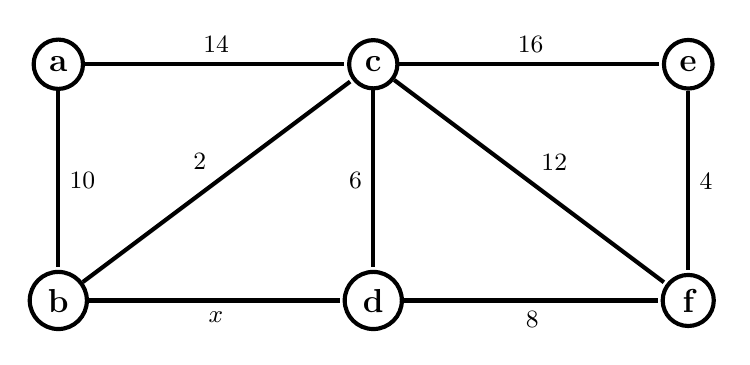
\begin{tikzpicture}[-,>=stealth,shorten >=1pt,auto,
  main node/.style={circle,draw,font=\large\bfseries}, line width=1.5pt]
\node[main node] (a) at (1,1.5) {a};
\node[main node] (b) at (1,-1.5) {b};
\node[main node] (c) at (5,1.5) {c};
\node[main node] (d) at (5,-1.5) {d};
\node[main node] (e) at (9,1.5) {e};
\node[main node] (f) at (9,-1.5) {f};

\path[every node/.style={font=\small}]
(a) edge node {10} (b)
(a) edge node {14} (c)
(b) edge node {2} (c)
(b) edge[below] node {$x$} (d)
(c) edge[left] node {6} (d)
(c) edge[above] node {16} (e)
(d) edge[below] node {8} (f)
(e) edge node {4} (f)
(c) edge node {12} (f);
\end{tikzpicture}
\end{center}

For hvilke værdier af $x$ er kanten \{{\bf b},{\bf d}\} med i det mindste udspændende træ?
\fleresvar
\mulighederstart
\svar $x=1$ \korrekt
\svar $x=3$ \korrekt
\svar $x=5$ \korrekt
\svar $x=7$
\svar $x=9$
\svar $x=11$
\svar $x=13$
\mulighederslut

\forklaring{
Man kan køre Kruskal for hvert valg af $x$. Man kan alternativt observere at Prim's algoritme med startknude $d$ inkluderer kanten \{{\bf b},{\bf d}\} hvis $x<6$. Hvis $x>6$ inkluderes i stedet kanterne \{{\bf c},{\bf d}\} og \{{\bf b},{\bf c}\}, dvs. \{{\bf b},{\bf d}\} inkluderes ikke.
}



\spoergsmaal{Disjunkte mængder}
Vi betragter trærepræsentationer af disjunkte mængder (eng.~\emph{disjoint sets}), som beskrevet i CLRS sektion 19.3, ved brug af \emph{weighted-union} heuristikken uden brug af stiforkortning.
Antag at $n$ og $m$ er store heltal (ikke begrænset af nogen konstant) hvor $m < n - 1$.
En algoritme laver $n$ kald til {\sc Make-Set}, og $m$ kald til {\sc Union}.
Hvad gælder for køretiden af et kald til {\sc Find-Set}$(x)$?
\fleresvar
\mulighederstart
\svar Tiden er $\Omega(\log n)$ for alle $x$
\svar Tiden er $O(\log n)$ for alle $x$\korrekt
\svar Tiden er $\Omega(\log m)$ for alle $x$
\svar Tiden er $O(\log m)$ for alle $x$\korrekt
\mulighederslut
\forklaring{ Højden af et træ med $k$ knuder er højst $\log k$ på grund af weighted-union heuristikken. Hvis vi laver $m$ {\sc Union} operationer kan der højst være $m+1$ elementer i hvert træ, dvs.~tiden er $O(\log m)$ hvilket også er $O(\log n)$ da $m<n$.
Hvis $x$ er i en komponent af størrelse 1 (der findes mindst én sådan komponent) så er tiden for {\sc Find-Set}$(x)$ konstant, dvs.~ikke $\Omega(\log n)$ eller $\Omega(\log m)$.
}



\spoergsmaal{Korteste veje}
Betragt følgende vægtede graf $G=(V,E)$:
\begin{center}
  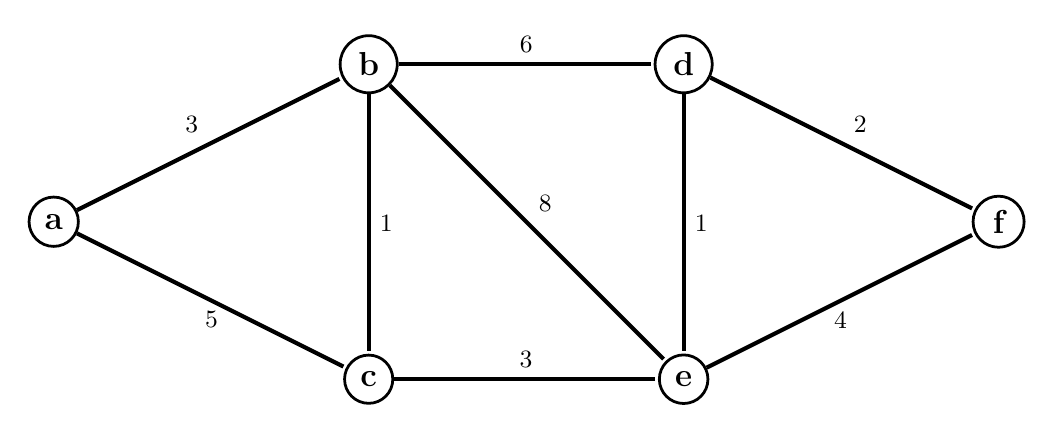
\begin{tikzpicture}[-,>=stealth,shorten >=1pt,auto,
      main node/.style={circle,draw,font=\large\bfseries,line width=1pt}, line width=1.5pt]
  \node[main node] (a) at (0,0) {a};
  \node[main node] (b) at (4,2) {b};
  \node[main node] (c) at (4,-2) {c};
  \node[main node] (d) at (8,2) {d};
  \node[main node] (e) at (8,-2) {e};
  \node[main node] (f) at (12,0) {f};
  \path[every node/.style={font=\small}]
  (a) edge node {3} (b)
  (a) edge[below] node {5} (c)
  (b) edge node {1} (c)
  (b) edge node {6} (d)
  (b) edge node {8} (e)
  (c) edge node {3} (e)
  (d) edge node {1} (e)
  (d) edge node {2} (f)
  (e) edge[below] node {4} (f);
  \end{tikzpicture}
\end{center}

Hvor mange kanter er der i den korteste vej (eng.~\emph{shortest path}) fra knude {\bf a} til knude~{\bf f}?
\etsvar
\mulighederstart
\svar 3 kanter
\svar 4 kanter
\svar 5 kanter \korrekt
\svar 10 kanter
\svar 11 kanter
\svar 12 kanter
\mulighederslut

\forklaring{
Grafen er uorienteret, dvs.~i en kantlisterepræsentation er der to kanter mellem hvert par af forbundne knuder. 
Kør Dijkstra på kantlisterepræsentationen med startknude A. 
Det giver den korteste vej A--B--C--E--D--F, som har 5 kanter. 
(Længden, dvs. den totale vægt af den korteste vej, er 10.)
}



\spoergsmaal{Valg af algoritme}
Vi ønsker at finde en sti gennem et 2-dimensionelt gitter fra en startposition $S$ til en slutposition $T$, der har en så lav omkostning som muligt.

\begin{center}    
\begin{tikzpicture}[scale=0.5, line cap=round, line join=round]
  % Grid size: 16 columns (x=0..16), 8 rows (y=0..8)
  % Coordinate system: (0,8) is top-left corner; (16,0) is bottom-right corner.

  % Light grid (optional)
  \draw[gray!25, very thin] (0,0) grid (10,6);

  % Mark start and goal cells
  \node[draw, circle, inner sep=1.5pt] at (0.5,5.5) {\scriptsize S};
  \node[draw, circle, inner sep=1.5pt] at (9.5,0.5) {\scriptsize T};

  \node at (2.5,5.5) {\scriptsize -2};
  \node at (4.5,4.5) {\scriptsize -1};
  \node at (1.5,2.5) {\scriptsize -2};
  \node at (3.5,1.5) {\scriptsize -2};
  \node at (8.5,3.5) {\scriptsize -1};
  \node at (7.5,0.5) {\scriptsize -1};
  \begin{scope}[on background layer]
 \draw[cyan]
    (0.5,5.5) -- (2.5,5.5) -- (2.5,4.5) -- (7.5,4.5) -- (7.5,3.5) -- (9.5,3.5)
    -- (9.5,0.5);
    \end{scope}
\end{tikzpicture}
\end{center}

I hvert skridt kan man flytte sig én position horisontalt eller vertikalt hvilket har en omkostning på~1.
Nogle celler indeholder et negativt tal: Går man til en sådan celle reduceres omkostningen svarende til størrelsen af tallet.
Den viste sti har en omkostning på 10: Der er 14 skridt og derfra trækkes 2, 1 og 1.
Den billigste sti har en omkostning på 9.
Hvilken af nedenstående algoritmer er mest egnet til at være en del af en algoritme der løser dette problem?
\etsvar
\mulighederstart
\svar Bellman-Ford algoritmen \korrekt
\svar Dijkstra's algoritme
\svar Longest Common Subsequence algoritmen
\svar Prim's algoritme
\svar Rod Cutting algoritmen
\mulighederslut
\forklaring{Problemet kan udtrykkes som et korteste-vej problem på en graf defineret ud fra gitteret. De negative bidrag kan modelleres som en kant internt i hver celle. Da der er negative kantvægte kan vi ikke bruge Dijkstra's algoritme men er nødt til at bruge den langsommere Bellman-Ford.
}




\spoergsmaal{Nærmeste par af punkter}
I CLRS digitalt kapitel 33, sektion 4, præsenteres en del-og-hersk algoritme med køretid $O(n \log n)$ til at finde nærmeste par af punkter i en mængde af 2-dimensionelle punkter.
Algoritmen starter med at sortere punkterne efter $y$-koordinat i tid $O(n \log n)$ og løser derefter problemet med en rekursiv algoritme.
Antag nu at algoritmens input allerede er sorteret således at sorteringsskridtet ikke behøves.
Hvad gælder for køretiden af den rekursive del af algoritmen, altså uden sorteringsskridtet?
\etsvar
\mulighederstart
\svar For alle input kører algoritmen i tid $\Theta(\log n)$
\svar For alle input kører algoritmen i tid $\Theta(n)$
\svar For alle input kører algoritmen i tid $\Theta(n \log n)$ \korrekt
\svar For alle input kører algoritmen i tid $\Theta(n^2)$
\mulighederslut
\forklaring{ Rekursionsligningen der bestemmer den rekursive algoritmes køretid er stadig $T(n) = 2 T(n/2) + \Theta(n)$, der har løsningen $T(n) = \Theta(n \log n)$.
}



\spoergsmaal{Længste fælles delsekvens}
Hvor lang er længste fælles delsekvens af strengene {\tt AABBCDAAB} og {\tt ABDAACBB}?
\etsvar
\mulighederstart
\svar Længde 1
\svar Længde 2
\svar Længde 3
\svar Længde 4
\svar Længde 5
\svar Længde 6\korrekt
\svar Længde 7
\mulighederslut
\forklaring{Kør LCS algoritmen fra CLRS:

\begin{center}
\begin{tabular}{c|c|c|c|c|c|c|c|c|c||}
    &   & A & B & D & A & A & C & B & B\\
    \hline
     & 0 & 0 & 0 & 0 & 0 & 0 & 0 & 0 & 0\\
     \hline
    A & 0 & $\nwarrow1$ & $\leftarrow1$ & $\leftarrow1$ & $\nwarrow1$ & $\nwarrow1$ & $\leftarrow1$ & $\leftarrow1$ & $\leftarrow1$ \\
    A & 0 & $\nwarrow1$ & $\uparrow1$ & $\uparrow1$ & $\nwarrow2$ & $\nwarrow2$ & $\leftarrow2$ & $\leftarrow2$ & $\leftarrow2$ \\
    B & 0 & $\uparrow1$ & $\nwarrow2$ & $\leftarrow2$ & $\uparrow2$ & $\uparrow2$ & $\uparrow2$ & $\nwarrow3$ & $\nwarrow3$ \\
    B & 0 & $\uparrow1$ & $\nwarrow2$ & $\uparrow2$ & $\uparrow2$ & $\uparrow2$ & $\uparrow2$ & $\nwarrow3$ & $\nwarrow4$ \\
    C & 0 & $\uparrow1$ & $\uparrow2$ & $\uparrow2$ & $\uparrow2$ & $\uparrow2$ & $\nwarrow3$ & $\uparrow3$ & $\uparrow4$ \\
    D & 0 & $\uparrow1$ & $\uparrow2$ & $\nwarrow3$ & $\leftarrow3$ & $\leftarrow3$ & $\uparrow3$ & $\uparrow3$ & $\uparrow4$ \\
    A & 0 & $\nwarrow1$ & $\uparrow2$ & $\uparrow3$ & $\nwarrow4$ & $\nwarrow4$ & $\leftarrow4$ & $\leftarrow4$ & $\uparrow4$ \\
    A & 0 & $\nwarrow1$ & $\uparrow2$ & $\uparrow3$ & $\nwarrow4$ & $\nwarrow5$ & $\leftarrow5$ & $\leftarrow5$ & $\leftarrow5$ \\
    B & 0 & $\uparrow1$ & $\nwarrow2$ & $\uparrow3$ & $\uparrow4$ & $\uparrow5$ & $\uparrow5$ & $\nwarrow6$ & $\nwarrow6$ \\
    \hline
\end{tabular}
\end{center}

En LCS er {\tt ABDAAB}, der har længde 6.
}




\spoergsmaal{Arbejde og spand}
Betragt følgende parallelle algoritme, der finder maksimum i et array $A[1\!:\!n]$ ved divide-and-conquer.

\begin{codebox}
\Procname{$\proc{Parallel-Max}(A, p, q)$}
\li \If $p == q$
\li \Then \Return $A[p]$
\li \Else
\li     $mid \gets \lfloor (p+q)/2 \rfloor$
\li     \Spawn $m_1 \gets \proc{Parallel-Max}(A, p, mid)$
\li     $m_2 \gets \proc{Parallel-Max}(A, mid+1, q)$
\li     \Sync
\li     \If $m_1 > m_2$
\li     \Then \Return $m_1$
\li     \Else \Return $m_2$\End
\end{codebox}

\noindent
Antag at $n = q-p+1$. Hvad er algoritmens arbejde (eng.~\emph{work}) og spand (eng.~\emph{span})?
\etsvar
\mulighederstart
\svar Arbejde $T_1=\Theta(\log n)$, spand $T_\infty=\Theta(\log n)$
\svar Arbejde $T_1=\Theta(\log n)$, spand $T_\infty=\Theta(n)$
\svar Arbejde $T_1=\Theta(n)$, spand $T_\infty=\Theta(\log n)$ \korrekt
\svar Arbejde $T_1=\Theta(n)$, spand $T_\infty=\Theta(n)$
\svar Arbejde $T_1=\Theta(n \log n)$, spand $T_\infty=\Theta(\log n)$
\svar Arbejde $T_1=\Theta(n \log n)$, spand $T_\infty=\Theta(n)$
\mulighederslut

\forklaring{
Hver rekursion deler input i to halvdele og udfører konstant ekstra arbejde.
Rekursionsligningn for arbejde er
$T_1(n)=2T_1(n/2)+O(1)=\Theta(n)$.
Spandet bestemmes af den længste afhængighedskæde:
$T_\infty(n)=T_\infty(n/2)+O(1)=\Theta(\log n)$.
Algoritmen har altså lineært arbejde og logaritmisk spand.
}




\multiplechoiceslut

\newpage

\section*{Skriftlige opgaver}\label{sec:written}

{\bf Skriftlige opgaver} afleveres som et Word dokument i ITX systemet.
Der er mulighed for at tegne og skrive på tablet, og indsætte i dokumentet.
\begin{itemize}
    \item Brug \emph{én side til hvert delspørgsmål, i samme rækkefølge som i opgavesættet.} 
    \item Delspørgsmålets nummer/bogstav (fx 19 eller 20.a) skal fremgå.
\end{itemize}


\section{Huffman træer (4\%)}

Vi betragter algoritmen til konstruktion af Huffman koder i CLRS sektion 15.3.

\punkt{}{Tegn Huffman træet som algoritmen beregner for alfabetet $C =\{A,E,I,O,U,Y\}$ med frekvenser $f_A=4$, $f_E=1$, $f_I=3$, $f_O=7$, $f_U=6$, $f_Y=1$.
Det er ikke nødvendigt at angive labels (0 og 1) på kanterne, men angiv frekvenser i blade såvel som indre knuder (se eksempel i CLRS sektion~15.3).}

\forklaring{Algoritmen beregner dette træ (tegnet uden 0-1 labels på kanterne):\medskip
\begin{center}
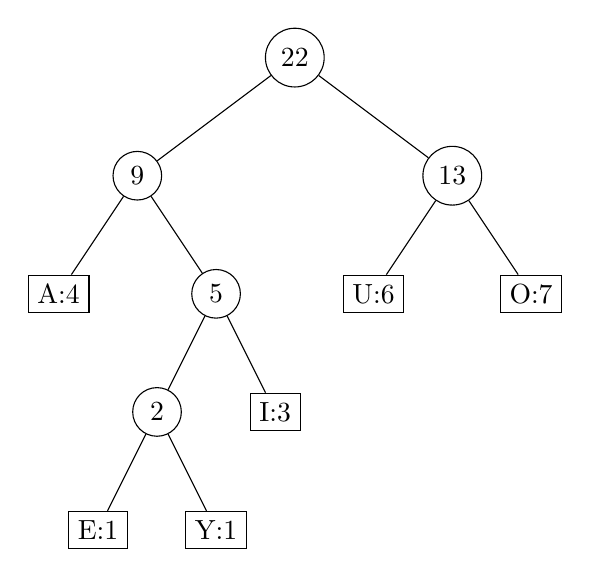
\begin{tikzpicture}[
  level distance=1.5cm,
  level 1/.style={sibling distance=4cm},
  level 2/.style={sibling distance=2cm},
  level 3/.style={sibling distance=1.5cm}
]
\node[circle,draw]{22}
  child {node[circle,draw]{9}
    child {node[rectangle,draw]{A:4}}
    child {node[circle,draw]{5}
      child {node[circle,draw]{2}
        child {node[rectangle,draw]{E:1}}
        child {node[rectangle,draw]{Y:1}}
      }
      child {node[rectangle,draw]{I:3}}
    }
  }
  child {node[circle,draw]{13}
    child {node[rectangle,draw]{U:6}}
    child {node[rectangle,draw]{O:7}}
  };
\end{tikzpicture}
\end{center}
}




\section{Største fælles præfixsum (12\%)}

For et array $S[1\!:\!n]$ defineres en \emph{præfixsum} af $S$ som et tal på formen $\sum_{i=1}^jS[i]$, for $j\in\{0,1,\ldots,n\}$.
I denne opgave er vi givet tre arrays $A[1\!:\!n],B[1\!:\!n],C[1\!:\!n]$, som alle indeholder positive heltal.
Vi ønsker at finde det største tal $x$ som er en præfixsum af både $A$, $B$ og $C$.
Med andre ord skal $x$ kunne skrives som $x=\sum_{i=1}^aA[i]=\sum_{i=1}^bB[i]=\sum_{i=1}^cC[i]$ for indekser $a,b,c\in\{0,1,\ldots,n\}$.
Bemærk at disse indekser $a,b,c$ gerne må være forskellige.

\punkt{a)}
{Lad $A=\langle 1,2,3,4\rangle$, $B=\langle 3,2,3,4\rangle$ og $C=\langle 1,1,1,4\rangle$.
Hvad er den største fælles præfixsum? Argumentér kort for dit svar.}

\forklaring{Svaret er $3$, hvilket kan skrives som præfixsummer $1+2=3=1+1+1$ i hhv.~$A$, $B$ og $C$ (vi vælger $a=2$, $b=1$, $c=3$). Den eneste større præfikssum for $C$ er~7, som ikke er en præfikssum for $A$ eller $B$.}

\punkt{b)}
{Beskriv en algoritme som kan finde den største fælles præfixsum.
Input til algoritmen er de tre arrays $A,B,C$ og deres størrelse $n$.
Du kan evt.~skrive pseudokode, men det er også tilstrækkeligt med en klar og præcis beskrivelse i tekst.
For at få fuldt point skal køretiden være $O(n)$.}

\forklaring{
Vi kan løse problemet med en grådig algoritme (men noterer at der findes andre løsninger).
Vi definerer variable $x_A,x_B,x_C$, som til at starte med er summen af alle tal i hhv.~$A,B,C$.
Vi definerer også indekser $a=b=c=n$.
Hvis $x_A$ er skarpt større end $x_B$ eller $x_C$ trækker vi $A[a]$ fra $x_A$ og trækker $1$ fra $a$, og tilsvarende hvis $x_B$ eller $x_C$ er større end en af de andre.
Dette svarer til at fjerne det sidste tal i præfixsummen $x_A$.
Når $x_A=x_B=x_C$ returnerer vi denne værdi.
Dette sker senest efter $3n$ iterationer, hvor vi vil have $a=b=c=0$ og $x_A=x_B=x_C=0$.
Derfor er køretiden $O(n)$.
Det kan skrives sådan i pseudokode:

\begin{codebox}
\Procname{$\proc{LargestCommonPrefixSum}(A,B,C, n)$}
\li let $x_A=\sum_{i=1}^n A[i]$, $x_B=\sum_{i=1}^n B[i]$, $x_C=\sum_{i=1}^n C[i]$ and $a=b=c=n$
\li \While $x_A\neq x_B$ or $x_A\neq x_C$
\Do
\li     \If $x_A>x_B$ or $x_A>x_C$
\li     \Then $x_A=x_A-A[a]$
\li         $a=a-1$
\li     \ElseIf $x_B>x_A$ or $x_B>x_C$
     \li     \Then $x_B=x_B-B[b]$
\li         $b=b-1$
\li \Else
\li     $x_C=x_C-C[c]$
\li         $c=c-1$
\End
\End
\li \Return $x_A$
\end{codebox}
}


\punkt{c)}
{Argumentér for at algoritmen altid finder det korrekte svar.}

\forklaring{
Vi vedligeholder invarianten at alle tre værdier $x_A,x_B,x_C$ er større end eller lig med løsningen $x$.
Da alle tal i $A,B,C$ er positive, er invarianten sand i begyndelsen.
Hvis en af $x_A,x_B,x_C$, fx $x_A$, er større end en anden, kan vi altså konkludere fra invarianten at $x_A$ er for stor.
Dermed holder invarianten igen efter at vi har fjernet det sidste tal $A[a]$ fra $x_A$.
}


\section{Algoritmeanalyse (12\%)} \label{sec:last}

Lad $\proc{BinarySearch}(A, p, q, x)$ være nedenstående algoritme der implementerer binær søgning efter~$x$ i et array $A[p\!:\!q]$ i tid $O(\log n)$ hvor $p\leq q$ og $n = q-p+1$ er antal elementer med $n>1$.
Under antagelse af at $A[p\!:\!q]$ indeholder heltal sorteret i ikke-aftagende rækkefølge returnerer $\proc{BinarySearch}(A, p, q, x)$ {\sc true} hvis $x$ findes i $A[p\!:\!q]$ og {\sc false} ellers.

\begin{codebox}
\Procname{$\proc{BinarySearch}(A,p,q,x)$}
\li \While $p \le q$
\li \Do $mid \gets p + \lfloor (q-p)/2 \rfloor$
\li \If $A[mid] = x$
\li \Then \Return \const{true}
\li \Else \If $A[mid] < x$
\li \Then $p \gets mid + 1$
\li \Else $q \gets mid - 1$\End\End\End
\li \Return \const{false}
\end{codebox}

Et array $A[1\!:\!n]$ er \emph{strengt bitonisk} hvis der findes et indeks $i$ således at $A[1\!:\!i]$ er voksende og $A[i:n]$ er aftagende.
%
{\bf Eksempel:} $A_1 = \langle 1, 2, 3, 5, 2, 1, 0\rangle$ er strengt bitonisk fordi $A_1[1\!:\!4] = \langle 1, 2, 3, 5\rangle$ er voksende og $A_1[4:7] = \langle 5, 2, 1, 0\rangle$ er aftagende. $A_2 = \langle 1, 2, 3, 5, 2, 2, 0\rangle$ kan ikke være strengt bitonisk fordi der er to på hinanden følgende identiske værdier.

\punkt{a)}{Giv et eksempel på et strengt bitonisk array $A[1\!:\!n]$ og et element $x$ fra $A$ hvor $\proc{BinarySearch}(A, 1, n, x)$ returnerer \const{false} (selv om $x$ findes i $A$).}

\forklaring{
For $A = \langle 3, 2, 1\rangle$ og $x=1$ sammenlignes $x$ først med $2$ og derefter med $3$ i næste iteration.
\medskip
}

Lad $\proc{ReverseBinarySearch}(A, p, q, x)$ have samme funktionalitet som $\proc{BinarySearch}$, med den forskel at $A[p\!:\!q]$ antages at være \emph{omvendt} sorteret (ikke-voksende rækkefølge). Vi ser nu på følgende rekursive algoritme:
%
\begin{codebox}
\Procname{$\proc{BTS2}(A,p,q,x)$}
\li $mid \gets \lfloor (p+q)/2 \rfloor$
\li \If $A[mid]==x$
\li \Then \Return \const{true}
\End
\li \If $p \ge q$
\li \Then \Return \const{false}
\End
\li \If $A[mid] < A[mid+1]$
\Then
\li     \If \proc{BinarySearch}$(A,p,mid,x)$
\li     \Then \Return \const{true}
    \End
\li     \If \proc{BTS2}$(A,mid+1,q,x)$
\li     \Then \Return \const{true}
    \End
\li \Else
\li     \If \proc{ReverseBinarySearch}$(A,mid+1,q,x)$
\li     \Then \Return \const{true}
    \End
\li     \If \proc{BTS2}$(A,p,mid,x)$
\li     \Then \Return \const{true}
    \End
\End
\li \Return \const{false}
\end{codebox}
\punkt{b)}{Opskriv en rekursionsligning for worst-case køretiden $T(n)$ af $\proc{BTS2}$ på et input af længde $n$, og brug den til at udlede en asymptotisk øvre grænse for køretiden. Analysen skal være så præcis som muligt.}

\forklaring{
I værste fald findes $x$ ikke i $A[p\!:\!q]$, dvs.~algoritmen returnerer først efter både den binære søgning og det rekursive kald.
I dette tilfælde udføres konstant arbejde, én binær søgning på højst $n/2$
elementer (tid $O(\log n)$), samt ét rekursivt kald på højst $n/2$
elementer.
Dermed fås rekursionsligningen \(T(n)=T(n/2)+O(\log n)\).
Den kan løses med master method eller ved substitutionsmetoden med resultat
\(
T(n)=\Theta((\log n)^2)
\).
}

\punkt{c)}{Antag at $A[1\!:\!n]$ er strengt bitonisk. Argumentér for at $\proc{BTS2}(A, 1, n, x)$ returnerer {\sc true} hvis $x$ findes i $A[1\!:\!n]$ og {\sc false} ellers.}

\forklaring{
Lad $A[1\!:\!n]$ være strengt bitonisk med toppunkt $i$, dvs.~$A[1\!:\!i]$ er voksende og $A[i:n]$ aftagende.
For et givet interval $A[p\!:\!q]$ afgør testen
$A[mid] < A[mid+1]$ om $mid$ ligger på den voksende
eller den aftagende del.
Hvis $A[mid] < A[mid+1]$, er $A[p\!:\!mid]$ voksende,
og det er korrekt at anvende $\proc{BinarySearch}$ til at afgøre om $x$ er i $A[p\!:\!mid]$.
Ellers er $A[mid+1\!:\!q]$ aftagende,
og det er korrekt at anvende $\proc{ReverseBinarySearch}$ til at afgøre om $x$ er i $A[mid+1\!:\!q]$.
Hvis $x$ ikke findes i den monotone halvdel,
kan det kun ligge i den anden halvdel,
som behandles rekursivt.
Intervallet halveres i hvert skridt,
så ved induktion over intervallets størrelse
returnerer algoritmen {\sc true}
hvis og kun hvis $x$ findes i $A[1\!:\!n]$.
(Basistilfældet $p=q$ håndteres af linje 2--5.)
}

\label{page:last}
